%!TEX root = report.tex	
\begin{subfigure}{0.16\textwidth}
	\centering
	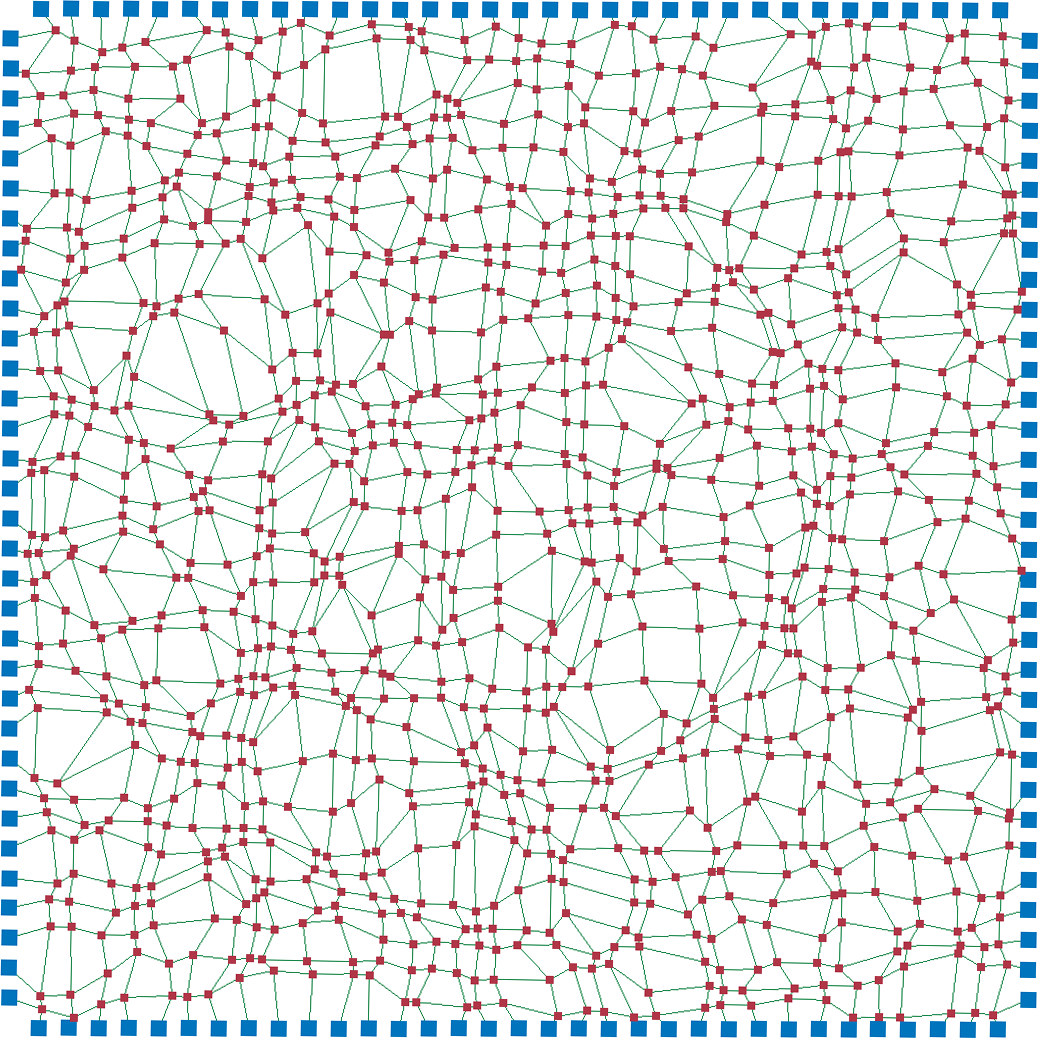
\includegraphics[
		width=\textwidth, 
		height=\textwidth, 
		keepaspectratio=true]
	{./img/results/1200_0_1_stretchGreaterThan_104_step_1}
	\caption{Step 0}
	\label{fig:experiment:stretchGreaterThanStrain:1}
\end{subfigure}	
\begin{subfigure}{0.16\textwidth}
	\centering
	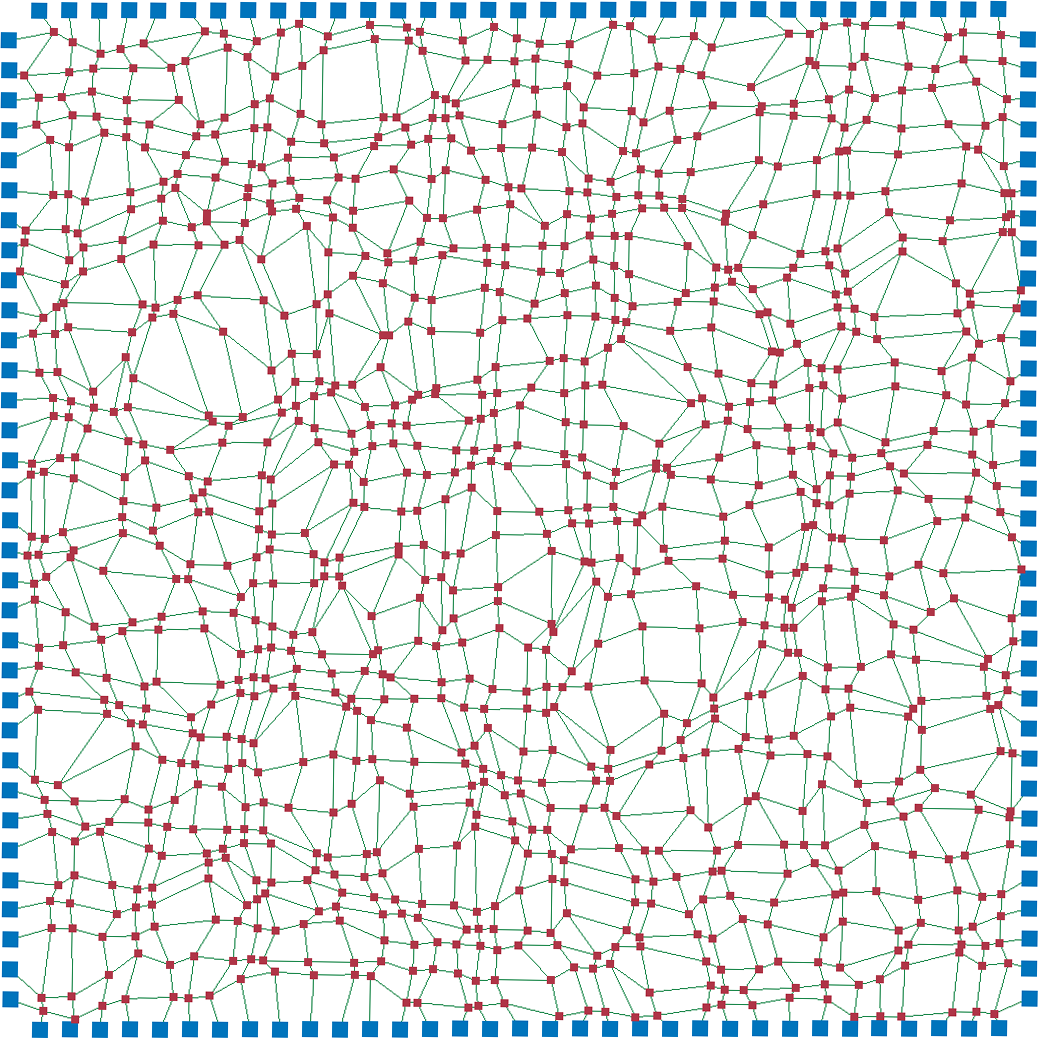
\includegraphics[
		width=\textwidth, 
		height=\textwidth, 
		keepaspectratio=true]
	{./img/results/1200_0_1_stretchGreaterThan_104_step_2}
	\caption{Step 1}
	\label{fig:experiment:stretchGreaterThanStrain:2}
\end{subfigure}		
\begin{subfigure}{0.16\textwidth}
	\centering
	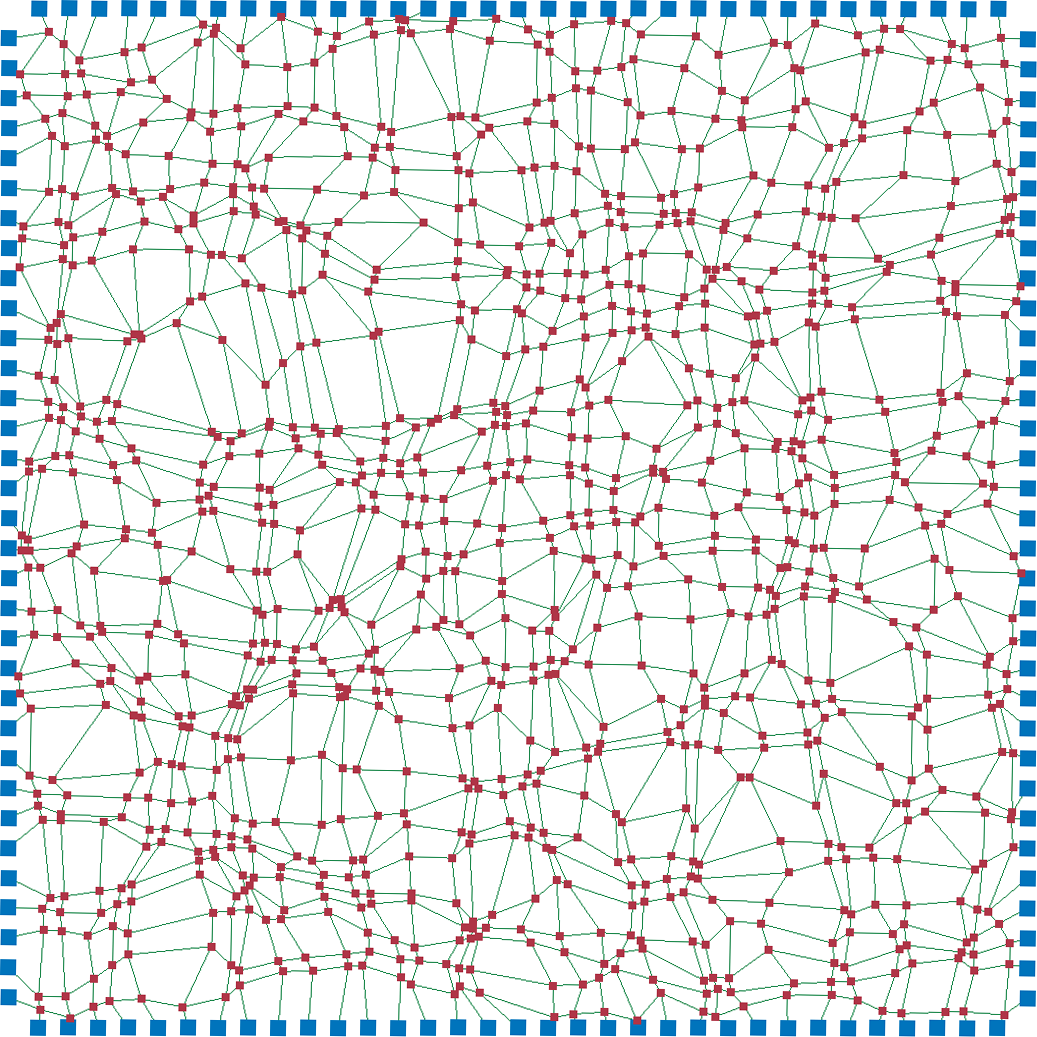
\includegraphics[
		width=\textwidth, 
		height=\textwidth, 
		keepaspectratio=true]
	{./img/results/1200_0_1_stretchGreaterThan_104_step_3}
	\caption{Step 2}
	\label{fig:experiment:stretchGreaterThanStrain:3}
\end{subfigure}			
\begin{subfigure}{0.16\textwidth}
	\centering
	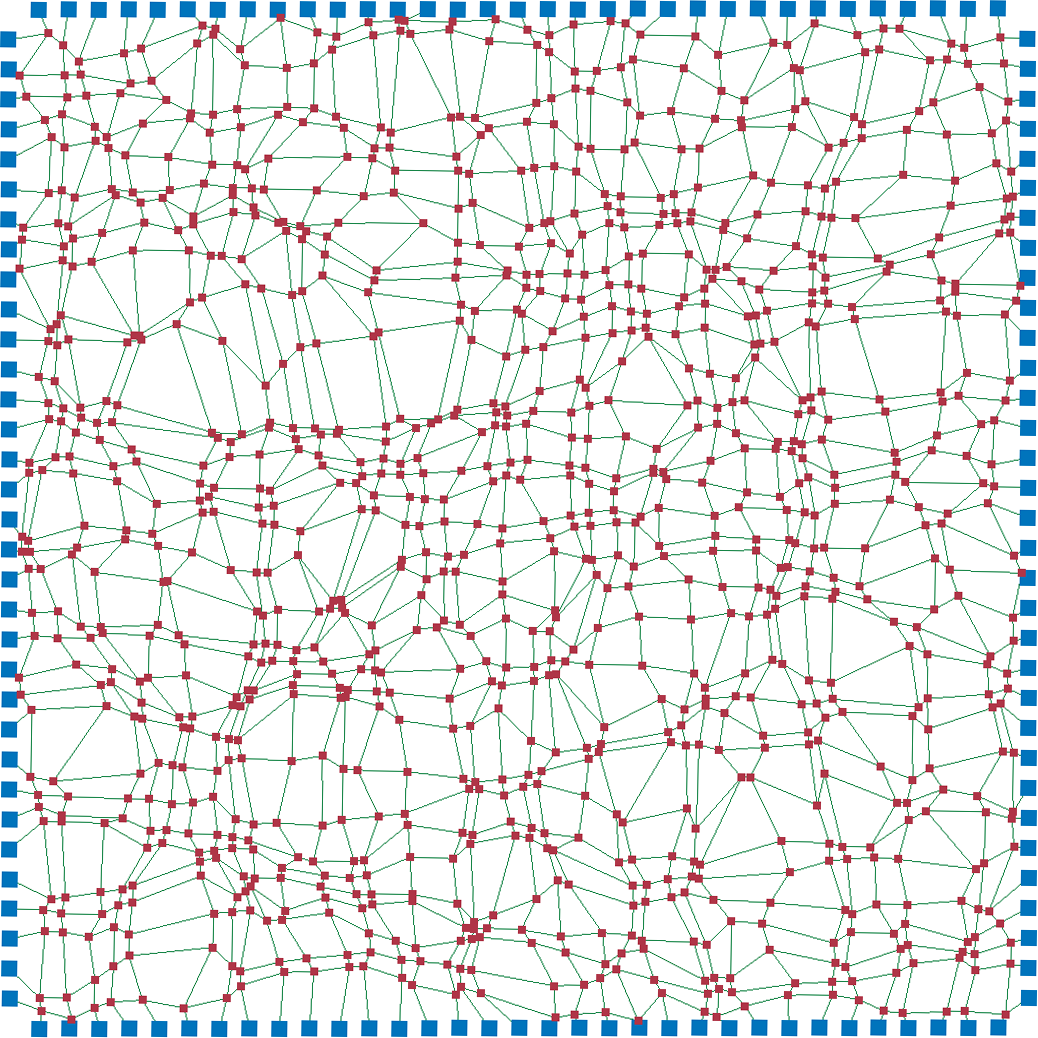
\includegraphics[
		width=\textwidth, 
		height=\textwidth, 
		keepaspectratio=true]
	{./img/results/1200_0_1_stretchGreaterThan_104_step_4}
	\caption{Step 3}
	\label{fig:experiment:stretchGreaterThanStrain:4}
\end{subfigure}				
\begin{subfigure}{0.16\textwidth}
	\centering
	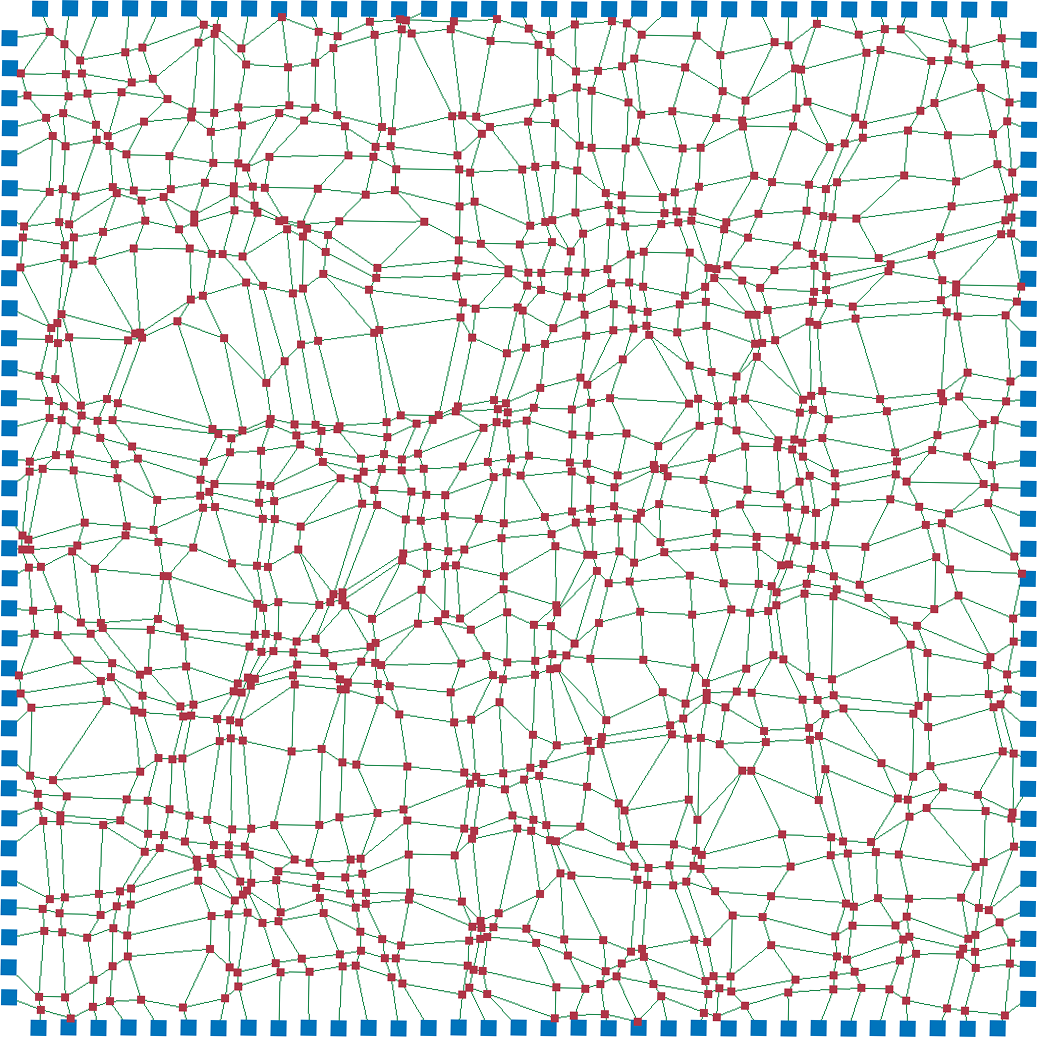
\includegraphics[
		width=\textwidth, 
		height=\textwidth, 
		keepaspectratio=true]
	{./img/results/1200_0_1_stretchGreaterThan_104_step_5}
	\caption{Step 4}
	\label{fig:experiment:stretchGreaterThanStrain:5}
\end{subfigure}